\documentclass{iopjournal}
\usepackage{amsmath,amssymb}
\usepackage{longtable,booktabs,array,calc}
\usepackage{textcomp}
\providecommand{\tightlist}{\setlength{\itemsep}{0pt}\setlength{\parskip}{0pt}}
\def\LTcaptype{table}

\begin{document}

\articletype{Paper}

\title{Accountable experiments: autonomy under contract}

\author{Petrus H. Zwart$^{1,*}$}
% TODO: co-authors, ORCID iDs (\orcid{...})

\affil{$^1$Molecular Biophysics and Integrated Bioimaging Division, Lawrence Berkeley National Laboratory, Berkeley, CA, USA}

\affil{$^*$Author to whom any correspondence should be addressed.}

\email{TODO@lbl.gov}

\keywords{accountable experiments, autonomous experimentation, distribution-free risk control, conformal prediction, adaptive sampling, hierarchical design, self-driving laboratories}

\begin{abstract}
Autonomous experiments decide where to measure, and every site they leave out enters the result as a prediction. An accountable experiment certifies every action: a site is measured because it was needed when the decision was made, or skipped because a stated claim covers it. The campaign runs under a contract fixed before it starts: a plan of sites at the finest resolution sought, the claims that justify a skip, a tolerance, an error budget and a confidence. A skip is made under one of two claims: the site holds nothing of interest, or its signal, or a quantity derived from it, can be predicted within tolerance from coarser measurements. Each level of the plan is set before its calibration draw, and a uniform draw from the level, taken after the model is frozen, bounds at the stated confidence the share of the level\textquotesingle s sites skipped under a false claim, whatever the model. The statistics are standard; the contribution is posing the experiment so that they apply inside a closed loop. On three fully measured datasets, an infrared map, a NaCl microdiffraction scan and a synthetic scattering phase map, levels exceeded their budget no more often than the stated confidence permits. A Gaussian process trusted on its own uncertainty misstated its share of wrong skips; on the synthetic map it stated at most 4 \% and skipped 11 \% to 41 \% of the sites wrongly. The model sets only the cost of a guarantee, and every decision can be replayed from the record.
\end{abstract}

\hypertarget{sec:1}{%
\section{Introduction}\label{sec:1}}

Autonomous decision engines are becoming routine in experimentation. At synchrotron beamlines, Gaussian-process surrogates choose the next sample position or composition, and measurement, analysis and decision run as one closed loop \cite{Noack2019,Noack2020,Yager2023}. Self-driving laboratories search formulation and composition spaces in the same way \cite{Burger2020,Nazeri2026}, and an autonomous laboratory synthesised 41 of 58 target inorganic compounds in 17 days \cite{Szymanski2023}. Probabilistic models recommend which strains to build next \cite{Radivojevic2020}, and laboratory automation keeps lowering the cost of handing experimental choices to machines \cite{Tom2024}.

Each decision to measure is also a decision to leave something unmeasured. Beam time, dose, reagents and sample lifetime are limited, and the sites left out of a map still enter it, as predictions. A closed-loop scattering study recently mapped the phases of a ternary polymer blend from 65 of 5151 grid compositions, so that 98.7 \% of the map is prediction \cite{Upreti2026}. As such decisions move from people to models, accountability becomes a requirement. Guidance on AI risk asks for traceable decisions and documented responsibility \cite{NIST2023}, regulation of high-risk systems requires automatic records of their operation \cite[Art. 12]{EU2024}, and audit frameworks ask for evidence that can be checked against stated expectations \cite{Raji2020}. For a measurement campaign the consequential decision is the skip, and the expectation to check is how often skips are wrong.

A surrogate model offers a rate of its own: its uncertainty states how likely each skip is to be wrong. The statement is the model\textquotesingle s about itself, and only the measurements it avoids could check it. Figure~\ref{fig:1} follows campaigns guided by Gaussian-process uncertainty on a fully measured diffraction scan; run at 90 \% to 99 \% intervals, they skipped 29 \% to 32 \% of their predictable sites wrongly where the intervals implied 1 \% to 10 \% (Fig. 1d).

\begin{figure}[tbp]
\centering
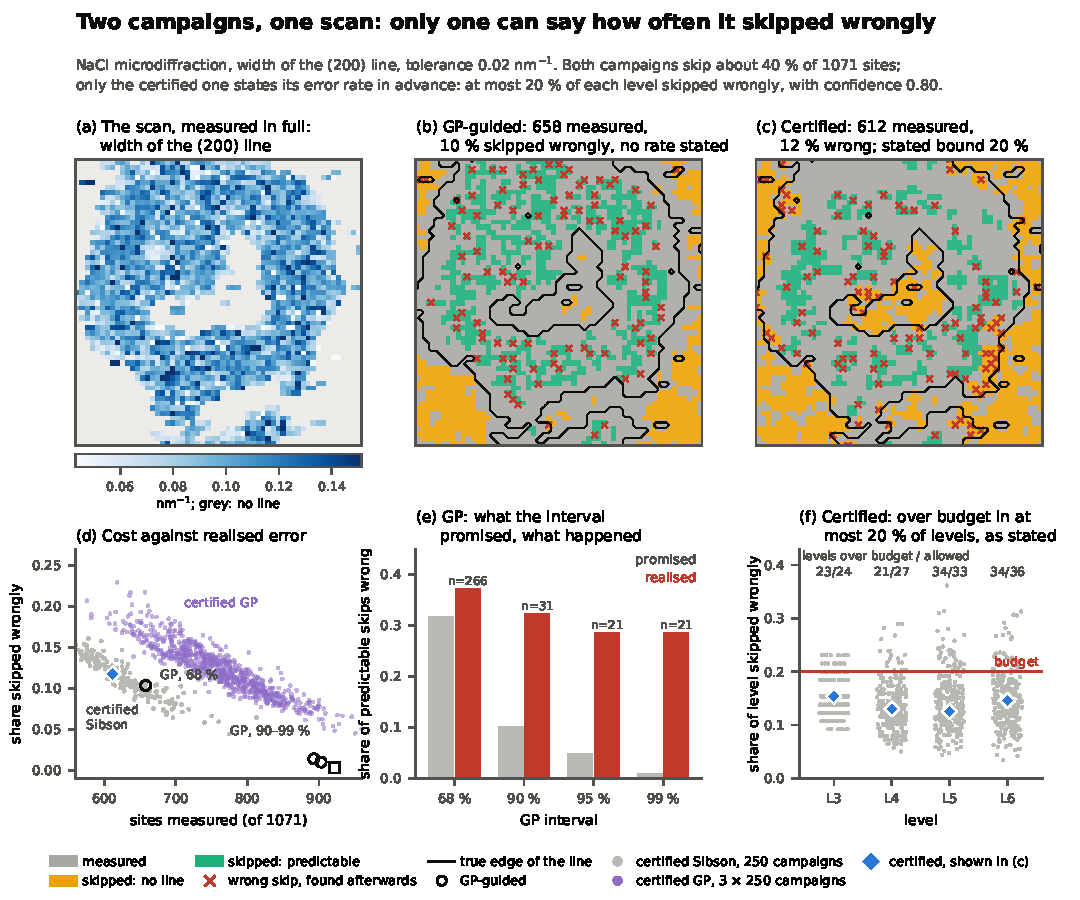
\includegraphics[width=\textwidth]{figures/fig_hook_compare}
\caption{Two campaigns on one fully measured NaCl microdiffraction scan, claim on the width of the (200) line (tolerance 0.02 nm\ensuremath{^{-1}}), each skipping about 40 \% of 1071 design sites. (a) The true (200) width. (b) A campaign guided by a Gaussian process refitted after each level, skipping where the model is sure the line is absent or its 68 \% interval on the width lies within the tolerance (SI 7). (c) The certified campaign of average cost; on each level, at most 20 \% of its sites skipped wrongly, with confidence 0.80 for that level. In (b) and (c), crosses mark wrong skips, found afterwards against the full scan: 10 \% and 12 \% of the sites of levels 3 to 6. (d) For campaigns run by the Gaussian-process rule at four interval levels, the share of predictable skips that the interval implies to be wrong and the share that was; numbers give the skips. (e) For 250 certified campaigns, the realised share of each level skipped wrongly against the budget of 20 \% (diamond: the campaign in (c)). Each level exceeds the budget with probability at most its picked failure probability, 0.12 on average; numbers give level runs over budget against the number expected.}\label{fig:1}
\end{figure}

A rate that can be checked needs claims that a measurement would settle. Two reasons justify a skip: the site holds nothing of interest, or its signal, or a quantity derived from it, can be predicted within tolerance from the sites already measured. Each reason is a claim about the site, and a wrong skip is a site covered by a false claim. Posed this way, skips come within reach of distribution-free risk control, which bounds the population rate of a chosen loss from a held-out sample for any predictor, with exchangeability of the calibration data as the only assumption \cite{Vovk2005,Bates2021,Angelopoulos2023,Angelopoulos2025}. Related constructions appear in imaging and power-grid screening (Section~\ref{sec:2}). A campaign strains that assumption, since every decision changes the data that calibrate the next.

This paper builds an accountable experiment for mapping campaigns, one that certifies every action. Any experiment declares in advance the most it will measure and the finest detail it seeks. The plan turns both into sites: those the experiment would measure if none could be skipped, at the finest spacing sought, and with them the sites for which every action is accounted. A site of the plan is measured because it was needed when the decision was made, or skipped because a stated claim covers it. The campaign runs under a contract fixed before it starts: the claims, the tolerance that makes a prediction correct, an error budget \ensuremath{\varepsilon} and a confidence c. The plan is divided into levels, and the coarsest levels are measured in full. At each finer level, a model fitted to the measured sites proposes which sites to skip, a uniform random sample of the level is measured for calibration, and its labels set how far the skips may go. The guarantee reads: at most a fraction \ensuremath{\varepsilon} of the level is skipped under a false claim, with probability at least c over the calibration draw. It holds for any predictor and any score that respect the order fit, freeze, draw, calibrate, decide; the model decides only how many measurements the guarantee costs. A plan may also be drawn up level by level within the declared limit, each level set from what was measured before its draw; the guarantee then concerns that level, and this study declares the plan in full. A nested, space-filling design \cite{Bridson2007} declared at the start serves image formation at every resolution.

The contributions are three. The first poses a mapping campaign as an accountable experiment: skips as claims a measurement would settle, a contract fixed in advance, a record from which every decision can be replayed, and guarantees of three forms built from existing risk-control results \cite{Angelopoulos2025,LauferGoldshtein2023}. The statistics are standard; the contribution is posing the experiment so that they apply. The second states the conditions that keep the guarantee valid inside the closed loop, a plan whose levels are set before their draws and an order of operations that forbids anticipation, and tests what breaking them does. The third is evidence on three fully measured datasets, an infrared map of a bioreef sample, a NaCl microdiffraction scan \cite{ALSNaCl} and a synthetic small-angle scattering phase map: levels exceeded their budgets no more often than the confidence permits, the model set the cost, the claim decided where measurements and wrong skips fell, and the same model trusted on its own uncertainty misstated its error rate.

\hypertarget{sec:2}{%
\section{Related work}\label{sec:2}}

\textbf{Adaptive mapping.} Scanning instruments spend most of their time on sites that add little to the final map, and adaptive acquisition puts that time where the map is uncertain or interesting. Gaussian-process regression drives autonomous small-angle scattering and diffraction mapping at synchrotron and neutron facilities \cite{Noack2019,Noack2020,Noack2021}, and steers robotic formulation of polymer blends through their scattering peak ratios \cite{Upreti2026}. Bayesian active learning maps phase diagrams of composition spreads on the fly at the beamline \cite{Kusne2020}. Dynamic sampling selects each new pixel of a point-wise image by the expected reduction in distortion and stops once an estimated distortion is reached \cite{Godaliyadda2018}. Scanning probe and electron microscopes run comparable loops of measurement, model update and choice of the next location \cite{Kalinin2021,Ziatdinov2022}. These methods judge the sites they leave out through the model that chose them.

\textbf{Distribution-free risk control.} Distribution-free inference attaches finite-sample statements to the output of an arbitrary predictor, with exchangeability of the calibration data as the only assumption \cite{Vovk2005,Angelopoulos2023}. Risk-controlling prediction sets bound the population rate of a chosen loss from a held-out sample \cite{Bates2021}, Learn-then-Test extends the bound to any family of decision rules searched in a fixed order or with a multiple-testing correction \cite{Angelopoulos2025}, and conformal risk control bounds an expected loss \cite{Angelopoulos2024}. Several risks can be controlled at once, and a path through a family of rules can be learned on part of the data \cite{LauferGoldshtein2023}. Conformal selection controls the false-discovery rate among the items a model selects \cite{Jin2023}, a statement close in spirit to a bound on wrong skips among the skipped sites. Its contribution on this side is to pose a skip as a claim about a site, so that the claims of a mapping campaign become the losses these methods control.

\textbf{Exchangeability in space.} Spatial data are dependent, and a calibration sample drawn from a map is exchangeable with the rest of the map only under conditions. Spatial conformal prediction obtains exact or approximate exchangeability from properties of the spatial process, for instance local approximate exchangeability around a prediction location for a broad class of processes \cite{Mao2024}. Design-based inference takes the opposite route and places the randomness in the sampling plan, so that statements about a finite population hold whatever the values in it \cite{Neyman1934,Cochran1977}. The campaign here follows the second route: a plan fixed level by level before each draw gives every level its population, and a uniform draw makes the calibration sample exchangeable with it, whatever the campaign did before, with no model of the spatial dependence.

\textbf{Adaptive sensing with guarantees.} Two recent lines of work bring calibrated uncertainty into the acquisition loop itself. Conformal intervals decide which pixels to re-scan in photon-limited scanning microscopy \cite{Ye2025} and when enough has been acquired in rate-adaptive sensing \cite{YangZhang2026}, both calibrated on data collected outside the running acquisition. Power-system security screening offers the closest construction outside imaging: a label-independent audit drawn from the current operating window certifies the violation rate among contingencies that a cheap surrogate lets the operator skip, and the surrogate affects the cost of the guarantee and leaves its validity untouched \cite{Manoharan2026}. The present work certifies each skip of a running scan by a claim, takes its calibration sample from the scan through the design, and checks every guarantee against fully measured truth.

\hypertarget{sec:3}{%
\section{Framework}\label{sec:3}}

\hypertarget{sec:3-1}{%
\subsection{Design and order of operations}\label{sec:3-1}}

An experiment declares before it starts the most it will measure and the finest detail it seeks. The plan, the sites it would measure if none could be skipped, carries both: its finest spacing sets the resolution of the final map, and its sites bound the measurements. The same plan serves the guarantee. A finite-sample guarantee about skipped sites needs a calibration sample that is exchangeable with the sites it speaks for \cite{Vovk2005}. Here the design creates that exchangeability. The population of every level is fixed before its calibration draw, and a uniform random draw from that population is the only source of randomness the guarantee relies on, as in design-based survey inference \cite{Neyman1934,Cochran1977}. The guarantee needs no model of the spatial field or of the noise.

A hierarchical Poisson-disk design \cite{Bridson2007} partitions the scan into nested levels of increasing density. Any plan whose levels are fixed before their draws would serve the guarantee equally: a grid, independent uniform points, or a level drawn up from the sites already measured, such as the neighbourhood of sites found interesting. The hierarchy serves image formation: the sites up to any depth contain every coarser depth and form an evenly spread design at that resolution, so each map builds on the coarser maps and interpolation has well-placed support. Nesting and spread set the cost of a guarantee and play no part in its validity. Each completed level also yields a map at the spacing of its sites, in which every site is measured or carries a certified prediction; a display map can be drawn afterwards with any interpolator. The coarsest levels form the seed and are measured in full. Each finer level is then processed once, in order, in five steps (Fig.~\ref{fig:2}):

\begin{enumerate}
\def\labelenumi{\arabic{enumi}.}
\tightlist
\item
  \emph{Fit.} The predictor and the scores are fitted on the sites measured so far.
\item
  \emph{Freeze.} Scores and predictor are fixed for every site of the level, and so is the decision rule: the family of thresholds, the budget and its split, and the number of calibration failures the level may allow.
\item
  \emph{Draw.} A calibration sample of \(m\) sites is drawn uniformly without replacement from the level, with randomness independent of everything else.
\item
  \emph{Calibrate.} The calibration sites are measured, their labels are evaluated against the frozen predictor, and the rule turns the labels into thresholds.
\item
  \emph{Decide.} Covered sites of the remainder are skipped and the others measured; every measured site joins the measured set for the next level.
\end{enumerate}

\begin{figure}[tbp]
\centering
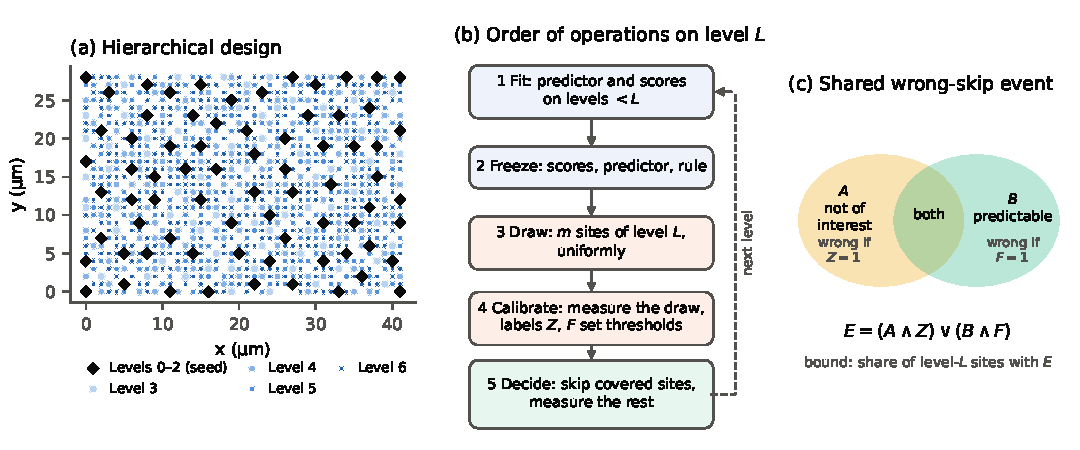
\includegraphics[width=\textwidth]{figures/fig1_schematic}
\caption{The workflow. (a) Hierarchical design of the IR map: levels 0--2 form the seed, and each finer level fills the gaps of the coarser ones. (b) The five steps on one level; the calibration draw is the only random element of the guarantee, and its labels are unseen until the rule is frozen. (c) The two claims: a skipped site is covered as not of interest (\(A\)), as predictable (\(B\)) or both, and the skip is wrong when a covering claim is false. The guarantee bounds the share of level-\(L\) sites at which the shared event \(E\) occurs.}\label{fig:2}
\end{figure}

Non-anticipation ties the steps together: nothing that shapes the guarantee on a level may depend on that level\textquotesingle s draw, except through the rule fixed in step 2. Three practices that look harmless break it, and Section~\ref{sec:5-1} shows each failing: refitting the scores on the calibration labels before the threshold is set, taking the calibration sample where the model is least sure, and keeping the most favourable of several draws. The condition concerns the draw and the rule. A score may use anything known before the draw, including physical models, other datasets or prior beliefs; a poor score costs measurements and leaves the guarantee intact.

Measuring one site must also leave the outcome of every other site unchanged. Radiation damage that spreads beyond the probed spot, or sample drift triggered by the measurement order, would let the draw alter the population it is meant to sample.

Given everything that precedes the draw of a level, its population, scores, labels and rule are fixed, so the guarantee holds conditionally on the history of the campaign and adaptivity across levels leaves it intact. Statements about several levels follow from the union bound; Appendix~\ref{app:A} states the conditions formally.

\hypertarget{sec:3-2}{%
\subsection{Claims and labels}\label{sec:3-2}}

A skip is useful only if it says something that a measurement could contradict. Two claims serve that purpose. The interest claim states that a site holds nothing of interest; its label \(Z(x) = 1\) marks a site whose measured spectrum meets the interest criterion of the dataset, such as a diffraction line standing clear of the noise. The interpolation claim states that a site is predictable; its label \(F(x) = 1\) marks a site where the prediction from the coarser levels misses the acceptance metric. The metric fixes what predictable means: agreement of the full spectrum within an envelope, or agreement of a quantity derived from it, such as a peak position or width, within a tolerance. Both labels are functions of the true spectrum, the one a single measurement returns, noise included, and of the frozen predictor. In a campaign they are known only at measured sites, and for this study they are known everywhere.

Each claim carries a score that orders the sites of a level from most to least safe to skip. The score has no other role: any function of the data available before the draw may serve, and its quality decides the number of measurements spent. The choice of metric decides more, since it sets where predictions fail and therefore where the campaign measures (Section~\ref{sec:5-5}).

\hypertarget{sec:3-3}{%
\subsection{The guarantee}\label{sec:3-3}}

A skip deserves a statement that a measurement could check. At level \(L\), claim \(j\) covers the sites whose frozen score lies at or below a threshold \(\tau_j\). A covered site is a wrong skip when the claim fails there, marked by \(B_j(x) = 1\). The controlled quantity is the rate of wrong skips over the level population:

\[
R_j(\tau_j) = N_L^{-1} \, \lvert \{x \in D_L : S_j(x) \le \tau_j,\ B_j(x) = 1\} \rvert
\]

The threshold comes from \(m\) sites drawn uniformly, without replacement, from the level after the scores are frozen and then measured. Let \(H\) count the failing sites in such a draw from a level in which \(\lfloor \varepsilon N_L \rfloor + 1\) sites fail. With \(k\) the largest integer for which

\[
P(H \le k) \le \delta
\]

every site scored below the \((k+1)\)-th failing calibration site is covered. The guarantee

\[
P\big(R_j(\hat\tau_j) \le \varepsilon\big) \ge 1 - \delta
\]

holds over the draw, for any score and any predictor \cite{Wilks1941,Bates2021,Angelopoulos2025}. The argument needs only a rate that grows with the threshold and a uniform draw; Appendix~\ref{app:A} gives it. The attained value \(\delta_L = P(H \le k)\), at most \(\delta\), is the failure probability the level carries, and \(c = 1 - \delta\) is the confidence of the contract. The statement concerns one level; all certified levels of a campaign hold together with probability at least \(1 - \sum_L \delta_L\) (Appendix~\ref{app:A}). Allowing no failure in the draw gives, in the binomial approximation, the smallest budget that \(m\) sites can certify, \(\varepsilon_{\min} = 1 - \delta^{1/m}\).

\hypertarget{sec:3-4}{%
\subsection{Forms of guarantee}\label{sec:3-4}}

Two claims justify a skip, and the rate a campaign must control depends on the question: wrong skips per claim, wrong skips overall, or wrong skips with one claim preferred. Each calls for its own form of guarantee. All forms rest on the shared wrong-skip event. With covers \(A_Z\) and \(A_F\) for the interest and interpolation claims,

\[
E(x) = \big(A_Z(x) \wedge Z(x)\big) \vee \big(A_F(x) \wedge F(x)\big)
\]

and \(R_E\) is its rate over the level. A site covered by both claims counts as wrong when either claim fails there.

\textbf{Per-claim budgets.} Each claim is calibrated on its own, with budget \(\varepsilon_j\) and failure probability \(\delta_j\), on one shared draw. A wrong skip fails at least one claim, so \(R_E \le R_a + R_b\), and the Bonferroni inequality gives

\[
P\big(R_E \le \varepsilon_a + \varepsilon_b\big) \ge 1 - \delta_a - \delta_b
\]

alongside a separate guarantee for each claim. The split leaves each claim a smaller budget at a higher confidence. Once \(\varepsilon_j\) falls below \(\varepsilon_{\min}\), no threshold exists and the level is measured in full.

\textbf{One budget along a path.} A single budget spends all of \(\varepsilon\) and \(\delta\) on \(R_E\). Two thresholds cannot be read off one draw by an order statistic, and Learn-then-Test supplies the remedy: search a family of thresholds fixed before any label is seen \cite{Angelopoulos2025}. Here the family is a path \(\lambda \mapsto (\tau_a(\lambda), \tau_b(\lambda))\), built from the frozen scores alone, along which both thresholds rise. The wrong-skip sets along such a path are nested, \(R_E(\lambda)\) grows with \(\lambda\), and the rule of Section~\ref{sec:3-3} applies with \(\lambda\) in place of the threshold (Appendix~\ref{app:B}). Two paths are used. The quantile path moves both thresholds through matching quantiles of their scores on the level. The priority path admits the claims in a set order: the first claim sweeps its quantiles before the second moves. A preference between the claims thereby enters the decision with the guarantee intact.

\textbf{Further forms.} The forms above share one recipe: scores frozen before the draw, a uniform calibration draw from the level, and a decision rule whose family of thresholds is fixed before the calibration labels are known. Any rule built this way inherits a finite-sample guarantee (Section~\ref{sec:6}), including a bound on a conditional rate (Appendix~\ref{app:C}). Table~\ref{tab:1} summarises the forms; SI 4 lists the conditions a new form must meet and a Monte Carlo acceptance check that every form here passes.

{\small
\begin{longtable}[]{@{}
  >{\raggedright\arraybackslash}p{(\columnwidth - 8\tabcolsep) * \real{0.2000}}
  >{\raggedright\arraybackslash}p{(\columnwidth - 8\tabcolsep) * \real{0.2000}}
  >{\raggedright\arraybackslash}p{(\columnwidth - 8\tabcolsep) * \real{0.2000}}
  >{\raggedright\arraybackslash}p{(\columnwidth - 8\tabcolsep) * \real{0.2000}}
  >{\raggedright\arraybackslash}p{(\columnwidth - 8\tabcolsep) * \real{0.2000}}@{}}
\caption{Forms of guarantee on the wrong-skip event of one level. Every form uses the same frozen scores and the same calibration draw.}\label{tab:1}\\

\toprule\noalign{}
\begin{minipage}[b]{\linewidth}\raggedright
Form
\end{minipage} & \begin{minipage}[b]{\linewidth}\raggedright
Guarantee, with probability at least the stated confidence
\end{minipage} & \begin{minipage}[b]{\linewidth}\raggedright
Budget
\end{minipage} & \begin{minipage}[b]{\linewidth}\raggedright
Given up
\end{minipage} & \begin{minipage}[b]{\linewidth}\raggedright
Suited to
\end{minipage} \\
\midrule\noalign{}
\endhead
\bottomrule\noalign{}
\endlastfoot
Per-claim budgets & \(R_a \le \varepsilon_a\) and \(R_b \le \varepsilon_b\); hence \(R_E \le \varepsilon_a + \varepsilon_b\) at \(1 - \delta_a - \delta_b\) & Split between the claims & Budget per claim; no threshold once \(\varepsilon_j < \varepsilon_{\min}\) & Reporting how often each reason for skipping fails \\
Quantile path & \(R_E \le \varepsilon\) at \(1 - \delta\) & Whole budget on \(R_E\) & Guarantee per claim; path shape set in advance & Bounding how often any skip fails \\
Priority path & \(R_E \le \varepsilon\) at \(1 - \delta\) & Whole budget on \(R_E\), spent on the claims in order & Guarantee per claim; a later claim may receive no budget & A set preference between the claims \\
Conditional rate (Appendix \ref{app:C}) & Failure rate among sites skipped by one claim \(\le \alpha\) at \(1 - \delta\) & One claim & Coverage at small \(m\): at \(m = 40\) it certifies nothing or more than half a level & Large calibration samples \\
\end{longtable}
}

\hypertarget{sec:3-5}{%
\subsection{What is claimed and what is checked}\label{sec:3-5}}

A reader of the record needs to know what each guarantee covers. Each guarantee of Sections~\ref{sec:3-3} and \ref{sec:3-4} concerns the design sites of one level and the predictor frozen for that level. Its probability is taken over the calibration draw of that level. It bounds how many skips fail, and the location of the failures is left open. It says nothing about points between design sites, nor about the final map, which draws on measurements made after the level was decided.

Two further statements accompany each level. The rate of wrong skips among the sites left after calibration, the remainder, follows from the same draw (Appendix~\ref{app:C}), and the calibration labels also bound the share of the level that the map from coarser levels predicts outside tolerance (SI 9).

A measurement is certified in another way. Each site was measured because the design placed it in the seed, the draw placed it in the calibration sample, or no claim covered it under the thresholds frozen for its level. This certification is exact, made at the time of decision and replayable; a measured site that hindsight finds predictable counts as a cost of the guarantee.

\hypertarget{sec:4}{%
\section{Experiments}\label{sec:4}}

\hypertarget{sec:4-1}{%
\subsection{Datasets}\label{sec:4-1}}

Every guarantee in this study can be checked, because each dataset is measured at every design site. Three datasets cover a simulation with known phase structure, a diffraction scan and a spectroscopic map.

\emph{Synthetic small-angle scattering map.} A forward model of a surfactant--oil--water formulation maps a composition in the triangle \(x + y \le 1\) to a scattering curve on 240 logarithmically spaced points between 0.005 and 0.32 \AA{}\ensuremath{^{-1}}. The model has a micellar phase, an ordered cubic phase, a hexagonal phase and an oil-rich emulsion, with smoothed transitions. A hierarchical Poisson-disk design on the unit square with nine levels, restricted to the triangle, gives 2118 sites. The interpolant uses mirror images across the walls of the triangle.

\emph{NaCl microdiffraction scan.} A raster of 3249 sites on a 0.25 mm stage grid, with curves of 1000 bins between 0.59 and 38.9 nm\ensuremath{^{-1}} \cite{ALSNaCl}. A seven-level design, snapped to the raster, gives 1071 sites.

\emph{Infrared map.} A bioreef sample mapped on 29 \ensuremath{\times} 42 pixels of 1 \ensuremath{\mu}m, with 1738 channels between 650 and 4000 cm\ensuremath{^{-1}}. Each spectrum is corrected for resonant Mie scattering pixel by pixel, and the window 1500--1850 cm\ensuremath{^{-1}}, which holds the amide and ester bands, is used. A seven-level design drawn on the physical rectangle and snapped to pixels gives 959 sites. SI 2 describes the correction and the design.

Figure~\ref{fig:3} shows each dataset as a map, with a site its claim accepts and one it rejects.

\begin{figure}[tbp]
\centering
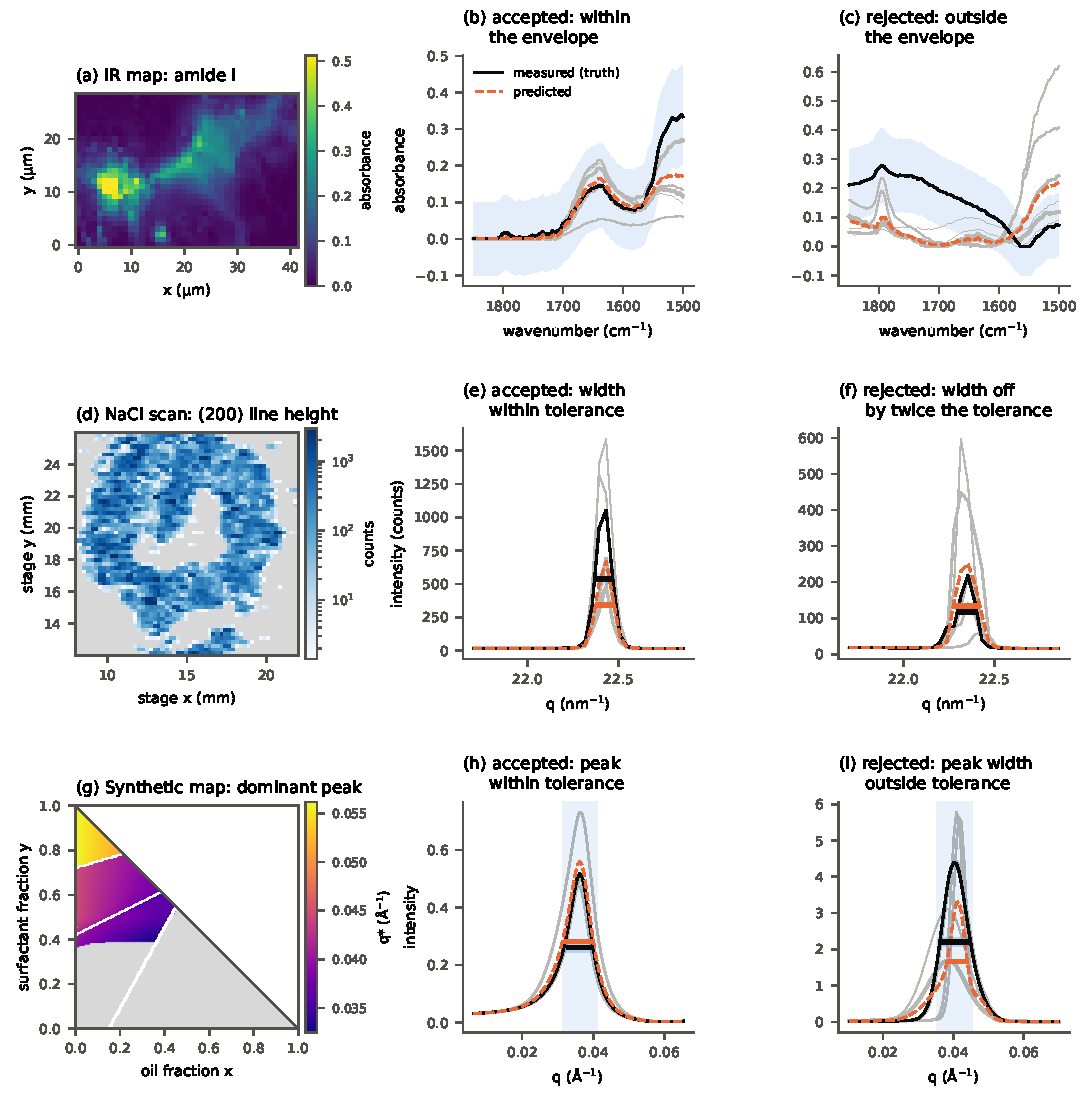
\includegraphics[width=\textwidth]{figures/fig_datasets_claims}
\caption{The three datasets and how their claims judge a prediction; rows: IR map, NaCl scan, synthetic map. Left column, the quantity the claims test: (a) amide-I absorbance, maximum over 1620--1690 cm\ensuremath{^{-1}} after scattering correction, 1 \ensuremath{\mu}m pixels; (d) height of the (200) line where it stands five times the noise above its baseline, grey where absent, the width (Fig. 1a) varying from pixel to pixel by more than the tolerance of the width claim; (g) position of the dominant peak where its prominence reaches 5, grey elsewhere, white lines: phase boundaries of the forward model. Middle and right columns: one site of a certified level that the claim accepts and one it rejects, predicted from the measured sites of the coarser levels by natural-neighbour weights (grey: neighbours, line width by weight; orange: prediction; black: measurement; shaded: tolerance). IR envelope claim: within 10 \% + 0.10 absorbance on average over channels above 0.02. NaCl width claim: widths at half maximum (bars) within 0.02 nm\ensuremath{^{-1}}. Synthetic peak claim: position within 0.005 \AA{}\ensuremath{^{-1}} (shaded column) and width within 0.001 \AA{}\ensuremath{^{-1}} (shaded bar).}\label{fig:3}
\end{figure}

\hypertarget{sec:4-2}{%
\subsection{Claims and tolerances}\label{sec:4-2}}

Each dataset carries one interest claim and one interpolation claim, fixed before any run.

{\small
\begin{longtable}[]{@{}
  >{\raggedright\arraybackslash}p{(\columnwidth - 4\tabcolsep) * \real{0.3333}}
  >{\raggedright\arraybackslash}p{(\columnwidth - 4\tabcolsep) * \real{0.3333}}
  >{\raggedright\arraybackslash}p{(\columnwidth - 4\tabcolsep) * \real{0.3333}}@{}}
\caption{Claims, fixed before any run.}\label{tab:2}\\

\toprule\noalign{}
\begin{minipage}[b]{\linewidth}\raggedright
Dataset
\end{minipage} & \begin{minipage}[b]{\linewidth}\raggedright
Interest: a site holds
\end{minipage} & \begin{minipage}[b]{\linewidth}\raggedright
Interpolation: the prediction from coarser levels meets
\end{minipage} \\
\midrule\noalign{}
\endhead
\bottomrule\noalign{}
\endlastfoot
Synthetic map & a dominant peak rising above its local baseline by at least five times that baseline & the dominant-peak position within 0.005 \AA{}\ensuremath{^{-1}} and its width within 0.001 \AA{}\ensuremath{^{-1}} \\
NaCl scan & the (200) line at 22.28 nm\ensuremath{^{-1}}, at least five times the noise above its local baseline & the (200) width within 0.02 nm\ensuremath{^{-1}}, about half a detector bin \\
IR map & absorbance of 0.1 or more in some channel of the window & every channel within 10 \% + 0.10 absorbance, on average over channels above 0.02 \\
\end{longtable}
}

A second setting of the IR map tightens the envelope to 10 \% + 0.01, with interest at 0.02 and channels counted above 0.005. Under it, interpolation rather than interest decides the cost. The choice of claim shapes the campaign as much as the budget does; Section~\ref{sec:5-5} and SI 6 compare six metrics on the three datasets.

\hypertarget{sec:4-3}{%
\subsection{Protocols}\label{sec:4-3}}

\textbf{Natural-neighbour protocol.} Natural-neighbour (Sibson) coordinates \cite{Sibson1981} predict the spectrum at a site as a weighted mean of the measured spectra around it. One set of weights per site serves every channel and every derived quantity. The weights are non-negative and sum to one, so a prediction from non-negative spectra is non-negative. The coordinates are computed exactly by clipping Voronoi cells (SI 1); outside the hull of the measured set, inverse-distance weights over the five nearest measured sites take over.

The interpolation score is one minus the probability of acceptance from a logistic regression. The regression is fitted by leave-one-out on the measured set (at most 120 sites), on the disagreement between natural neighbours in units of the acceptance metric and on the position. The interest score depends on the dataset. On the IR map it is the predicted maximum in the window, capped below the interest level, so that a site predicted to be of interest is never covered. On the two scattering datasets it is the probability of interest from a logistic regression on the predicted peak height above its baseline, the spread of that height over the five nearest measured sites and the distance to the nearest of them. The random scorer of Section~\ref{sec:5-4} assigns every site an independent uniform weight.

\textbf{Gaussian-process protocols.} Gaussian-process regression is the interpolator of choice for autonomous scattering experiments \cite{Noack2019,Noack2020}, and it offers a reason for every measurement: the posterior standard deviation is large where the measured set is far away in units of the length scale. The GP protocols place an isotropic squared-exponential kernel on the coordinates of the hierarchical design and evaluate the process only at design sites \cite{RasmussenWilliams2006}. The posterior mean, clipped at zero because every spectrum here is non-negative, predicts the full spectrum at a site, and the posterior standard deviation at unit output scale orders the sites for the interpolation claim. Both depend on the measured set through one set of linear weights, so the spectrum and any quantity derived from it come from the same fit, as with natural-neighbour coordinates. The interest claim keeps its score from the natural-neighbour protocol, which isolates the change of interpolator.

The length scale is set in three ways, each fixed before the calibration draw of a level: by maximum marginal likelihood on the leading principal-component scores of the measured spectra \cite{Balandat2020}, by the median nearest-neighbour spacing of the design through the finest level measured, or locally, through a Gibbs kernel whose length scale is the distance to the third-nearest measured site \cite{Gibbs1997,PaciorekSchervish2004}. SI 1 gives the details.

\textbf{Common settings.} Levels up to the second form the seed and are measured in full. Every finer level is calibrated on \(m = 40\) sites, or on the whole level when it is smaller. The guarantee on the shared wrong-skip rate is \(R_E \le 0.10\) at confidence 0.75 on the IR map and \(R_E \le 0.20\) at confidence 0.80 on the NaCl and synthetic maps. The per-claim form gives each claim half the budget at half the failure probability, so the union bound returns the same statement. Every rule uses the exact finite-population tail, and the threshold is placed at the score of the first calibration failure beyond those allowed.

{\small
\begin{longtable}[]{@{}
  >{\raggedright\arraybackslash}p{(\columnwidth - 2\tabcolsep) * \real{0.5000}}
  >{\raggedright\arraybackslash}p{(\columnwidth - 2\tabcolsep) * \real{0.5000}}@{}}
\caption{Exchangeable parts of a campaign.}\label{tab:3}\\

\toprule\noalign{}
\begin{minipage}[b]{\linewidth}\raggedright
Part
\end{minipage} & \begin{minipage}[b]{\linewidth}\raggedright
Options used
\end{minipage} \\
\midrule\noalign{}
\endhead
\bottomrule\noalign{}
\endlastfoot
Design & Hierarchical Poisson-disk design; seed of levels 0--2; 7 (NaCl, IR) or 9 (synthetic) levels \\
Interpolator & Natural-neighbour coordinates; Gaussian process with length scale by maximum likelihood, by design spacing or by local spacing \\
Interest score & Predicted maximum (IR); logistic on predicted peak height (NaCl, synthetic); random \\
Interpolation score & Logistic on neighbour disagreement; GP posterior standard deviation; random \\
Form of guarantee & Per-claim budgets; quantile path; priority path \\
Calibration & 40 sites per level, uniform without replacement, exact hypergeometric tail \\
\end{longtable}
}

\hypertarget{sec:4-4}{%
\subsection{Evaluation}\label{sec:4-4}}

A guarantee about a probability needs repetition to be checked. Each of 36 configurations was run as 250 campaigns that differ only in their calibration draws and, for the random scorer, in the score stream. Every certified level of every campaign gives one level check against the budget, and the checks over budget are compared with the number the picked failure probabilities lead one to expect (Section~\ref{sec:3-3}). For the first 20 campaigns of each configuration, the calibration draw was also repeated 1000 times on the recorded level populations, which isolates the randomness of the draw (SI 4, SI 5).

\hypertarget{sec:5}{%
\section{Results}\label{sec:5}}

All numbers below come from the run record: 36 configurations, each run as 250 independent campaigns with their own calibration draws (SI 5).

\hypertarget{sec:5-1}{%
\subsection{The guarantee holds}\label{sec:5-1}}

Checking a probability bound needs repeated campaigns against a known truth. Every certified level of every campaign was therefore checked against the fully measured truth (SI 5).

The picked failure probabilities \(\delta_L\) (Section~\ref{sec:3-3}) averaged 0.19 against a nominal 0.25 for the IR map and 0.11 to 0.12 against 0.20 for the NaCl and synthetic maps. The observed exceedances are to be compared with \(\delta_L\), and the four levels of a NaCl campaign hold together with probability at least about one half.

The record agrees with the guarantee at the picked failure probabilities: over the 32 statements whose budget can be exceeded on every level, observed exceedances lay between 0.88 and 1.11 times the number expected, and none exceeded it beyond chance (SI 5, Table S5.3). On the IR map at its original tolerance, three of the four levels hold too few failing sites for the budget to be reached. Repeating the calibration draw on the recorded level populations gives the same picture (Table S5.2).

Table~\ref{tab:4} gives one configuration per map: what was measured, why each site was skipped, and how the record compares with the guarantee. The guarantee bounds wrong skips as a share of all sites of a level; among the skipped sites alone the share is larger, up to 26.7 \% on the NaCl scan.

{\small
\begin{longtable}[]{@{}
  >{\raggedright\arraybackslash}p{(\columnwidth - 12\tabcolsep) * \real{0.1429}}
  >{\raggedright\arraybackslash}p{(\columnwidth - 12\tabcolsep) * \real{0.1429}}
  >{\raggedright\arraybackslash}p{(\columnwidth - 12\tabcolsep) * \real{0.1429}}
  >{\raggedright\arraybackslash}p{(\columnwidth - 12\tabcolsep) * \real{0.1429}}
  >{\raggedright\arraybackslash}p{(\columnwidth - 12\tabcolsep) * \real{0.1429}}
  >{\raggedright\arraybackslash}p{(\columnwidth - 12\tabcolsep) * \real{0.1429}}
  >{\raggedright\arraybackslash}p{(\columnwidth - 12\tabcolsep) * \real{0.1429}}@{}}
\caption{One guarantee per dataset: quantile path, natural-neighbour interpolation, 250 campaigns; counts are means per campaign. Wrong skips are given as a share of the sites on certified levels, the quantity the guarantee bounds, and as a share of the skipped sites. Expected exceedances are the sums of the picked failure probabilities over the level checks.}\label{tab:4}\\

\toprule\noalign{}
\begin{minipage}[b]{\linewidth}\raggedright
Dataset
\end{minipage} & \begin{minipage}[b]{\linewidth}\raggedright
Guarantee
\end{minipage} & \begin{minipage}[b]{\linewidth}\raggedright
Sites
\end{minipage} & \begin{minipage}[b]{\linewidth}\raggedright
Measured: seed / calibration / no claim
\end{minipage} & \begin{minipage}[b]{\linewidth}\raggedright
Skipped: not of interest / predictable / both
\end{minipage} & \begin{minipage}[b]{\linewidth}\raggedright
Wrong skips: count (share of sites / of skips)
\end{minipage} & \begin{minipage}[b]{\linewidth}\raggedright
Exceedances: observed / expected
\end{minipage} \\
\midrule\noalign{}
\endhead
\bottomrule\noalign{}
\endlastfoot
IR map & \(R_E \le 0.10\) at 0.75 & 959 & 73 / 160 / 62 & 37 / 228 / 399 & 34 (3.8 \% / 5.1 \%) & 49 / 190 (56 on reachable levels) \\
IR map, tight tolerance & \(R_E \le 0.10\) at 0.75 & 959 & 73 / 160 / 388 & 8 / 257 / 73 & 54 (6.1 \% / 15.9 \%) & 193 / 190 \\
NaCl scan & \(R_E \le 0.20\) at 0.80 & 1071 & 76 / 160 / 378 & 157 / 156 / 144 & 122 (12.3 \% / 26.7 \%) & 112 / 120 \\
Synthetic map & \(R_E \le 0.20\) at 0.80 & 2118 & 39 / 233 / 62 & 321 / 319 / 1144 & 270 (13.0 \% / 15.1 \%) & 161 / 170 \\
\end{longtable}
}

Breaking the order of operations breaks the guarantee (Section~\ref{sec:3-1}). On a level of 399 sites with informative scores, a budget of 0.10 and a picked failure probability of 0.206, the calibration draw was repeated 4000 times under several rules. With scores frozen before a uniform draw the budget was exceeded in 20.5 \% of draws, and so it was with a score that knew the true labels but was frozen before the draw: what the score knows changes the cost and leaves the guarantee intact. Rules that use the draw broke it. Thresholding on scores refitted to the calibration labels exceeded the budget in every draw, calibrating on the half of the level ranked least safe, as an active learner would, in 63 \%, and keeping the best of five draws in 69 \%. Setting the interpolation threshold on the calibration sites the interest threshold left uncovered exceeded it in 28.8 \%, where the priority path, which fixes the same preference in advance, stayed at 20.5 \%. Every form of Table~\ref{tab:1} kept its guarantee, and none was the least expensive on all three maps (Fig. S3; Table S3.1).

\hypertarget{sec:5-2}{%
\subsection{A model\textquotesingle s own uncertainty misstates its wrong skips}\label{sec:5-2}}

Decisions resting on a model\textquotesingle s stated error rate need that rate to hold. On the NaCl scan, a Gaussian process refitted after each level skipped a site when it was sure the line was absent, or when its 68 \% interval on the width lay within the tolerance (Fig.~\ref{fig:1}; SI 7). It measured 658 of 1071 sites and skipped 10 \% of the certified-level sites wrongly, inside the spread of the certified campaigns, which measured 614 \ensuremath{\pm} 56 sites with natural-neighbour interpolation and 745 to 777 with the Gaussian process as predictor (Fig. S7). Certifying the Gaussian process cost about 100 more measurements and bought a rate fixed in advance; the uncertified rate fell unevenly, 18 \% on the last level. At 68 \% intervals the implied and realised shares of wrong predictable skips came close, 32 \% and 37 \%; at 90 \% to 99 \% the intervals implied 1 \% to 10 \%, and 29 \% to 32 \% of 21 to 31 skips were wrong.

The comparison was repeated on all three maps with the Gaussian process of the certified campaigns in Section~\ref{sec:5-4}, which predicts the whole profile. A site was skipped under a claim when the posterior probability of a wrong skip was at most \ensuremath{\alpha}, for \ensuremath{\alpha} from 0.01 to 0.32, with the latent standard deviation, the predictive one, or the predictive one rescaled to the leave-one-out residuals of the measured sites (SI 7). Stated and realised shares of wrong skips disagreed in either direction (Fig.~\ref{fig:4}). On the synthetic map the process stated at most 4 \% and skipped 11 \% to 41 \% of the certified-level sites wrongly. Rescaling made it worse, and the reason is the one a uniform draw removes: the sites the process chose to measure were easier for it to predict than those it left out, and the scale fell to between 0.23 and 0.87 of its value. On IR the stated shares stayed below 10 \% and the realised ones below 5 \%, with 73 to 398 of 959 sites measured. On NaCl the process judged almost every site too uncertain to skip and measured 959 to 1070 of 1071.

The misstatement lay in the interpolation claim. On the synthetic map, sites skipped only because the line was judged absent were almost never wrong, 0 to 2 of 293 to 509; every other wrong skip failed the tolerance (SI 7). A rate stated by the model therefore says little about the rate realised, in size or direction. The certified campaigns at budgets from 0.05 to 0.30 realised on average less than their bound on every map; certified points pair a bound with a mean, uncertified points a stated expectation with a realisation.

\begin{figure}[tbp]
\centering
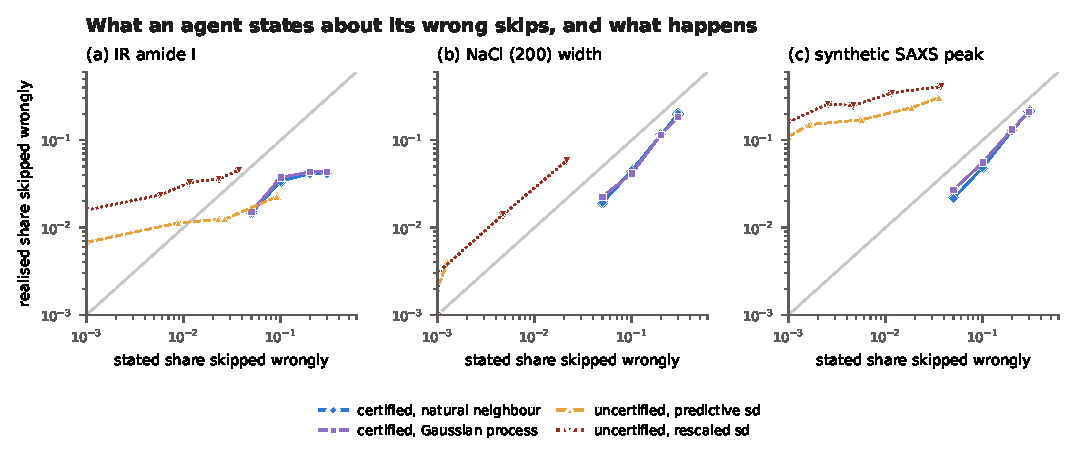
\includegraphics[width=\textwidth]{figures/fig_stated}
\caption{What an agent states about its wrong skips, and what happens. Stated against realised share of certified-level sites skipped wrongly, for certified campaigns with natural-neighbour (blue) and Gaussian-process (purple) prediction at budgets 0.05 to 0.30 (the bound against the mean over 20 or 8 campaigns) and for uncertified Gaussian-process campaigns at \ensuremath{\alpha} from 0.01 to 0.32 with latent, predictive or rescaled standard deviation; shares below 10\ensuremath{^{-}}\ensuremath{^{3}} are drawn at 10\ensuremath{^{-}}\ensuremath{^{3}}; grey: equality.}\label{fig:4}
\end{figure}

\hypertarget{sec:5-3}{%
\subsection{Every action certified}\label{sec:5-3}}

An instrument record becomes useful once every site of a map carries its reason. Figure~\ref{fig:5} shows one campaign of average cost per dataset under the quantile path with natural-neighbour interpolation, with every design site marked by the reason recorded for it and every wrong skip found against the fully measured truth.

In the campaigns shown, the wrong skips were 3.8 \% of the sites on certified levels of the IR map, against a budget of 0.10 per level, and 11.8 \% on NaCl and 11.6 \% on the synthetic map, against 0.20. The wrong skips of the synthetic map gather in two compact regions of the composition triangle; the guarantee bounds their rate on each level and leaves their location open (Section~\ref{sec:5-5}; SI 6).

In hindsight, the record shows which measurements every claim would have skipped wrongly (SI 8): 45 \% of the sites measured for want of a claim on the synthetic map, against 10 \% of sites drawn at random, and 47 \% against 35 \% on NaCl, where the width scatters from site to site by about the tolerance.

\begin{figure}[tbp]
\centering
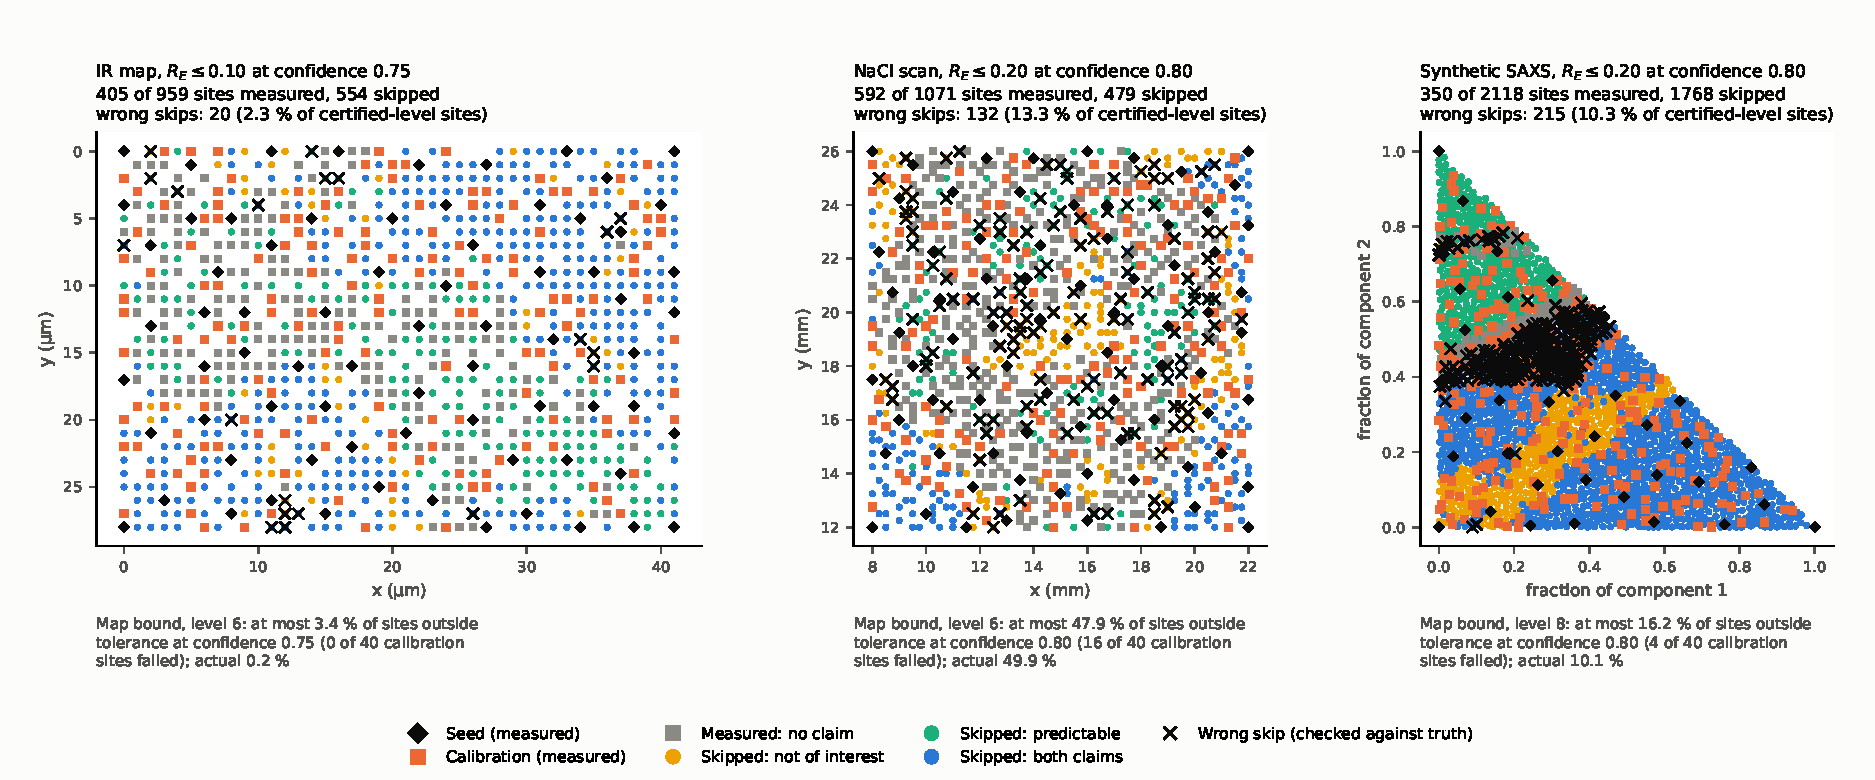
\includegraphics[width=\textwidth]{figures/fig5_maps}
\caption{Maps with reasons, one campaign of average cost per dataset (quantile path, natural-neighbour interpolation; NaCl: the campaign of Fig. 1c; the same campaigns as SI 8). Measured sites: seed (black diamonds), calibration (dark grey squares) and sites without a claim (light grey squares). Skipped sites: not of interest (yellow), predictable (green) and both (blue). Crosses: wrong skips against the fully measured truth. IR in micrometres, NaCl in stage millimetres, synthetic map in composition fractions.}\label{fig:5}
\end{figure}

\hypertarget{sec:5-4}{%
\subsection{The model sets the cost}\label{sec:5-4}}

Freedom in the choice of model has a price, paid in measurements. The quantile path was run with four interpolation protocols on each dataset at the nominal guarantees of Section~\ref{sec:5-1}: natural-neighbour interpolation with the logistic score, and Gaussian-process interpolation with the posterior standard deviation as score and three rules for the length scale (Section~\ref{sec:4-3}). At the original IR tolerance almost every site is interpolable and the interest claim alone sets the cost; at the tight tolerance interpolation decides.

A score that carries no information still yields a valid guarantee, at a price. A random scorer, an independent uniform weight per site and claim, exceeded the budget no more often than expected on every map and cost 1.4 to 3.2 times as many measurements as informed scores, 716 \ensuremath{\pm} 71 against 295 \ensuremath{\pm} 53 of 959 sites on IR (Fig.~\ref{fig:6}). The guarantee comes from the calibration draw; the score decides what it costs.

Every guarantee held, with exceedance counts on each map close to those the picked failure probabilities lead one to expect and none beyond chance (Fig.~\ref{fig:6}; Table S5.3).

The cost depends on the protocol and on the data (Fig.~\ref{fig:6}; Table S3.2). At the original IR tolerance the four protocols measured 273 \ensuremath{\pm} 31 to 295 \ensuremath{\pm} 53 of 959 sites with skipped sets overlapping by about 90 \%; at the tight tolerance they measured 621 \ensuremath{\pm} 70 to 799 \ensuremath{\pm} 40, and the Gaussian-process protocols shared a quarter to a third of their skips with natural-neighbour interpolation. On NaCl, the Gaussian-process protocols measured 745 to 777 of 1071 sites, against 614 \ensuremath{\pm} 56. On the synthetic map they measured between 1040 \ensuremath{\pm} 202 and 1443 \ensuremath{\pm} 133 of 2118 sites, against 334 \ensuremath{\pm} 26. The difference arises in the calibration draws: more failing calibration sites admit fewer skips at the same budget, and the guarantee is unchanged.

\begin{figure}[tbp]
\centering
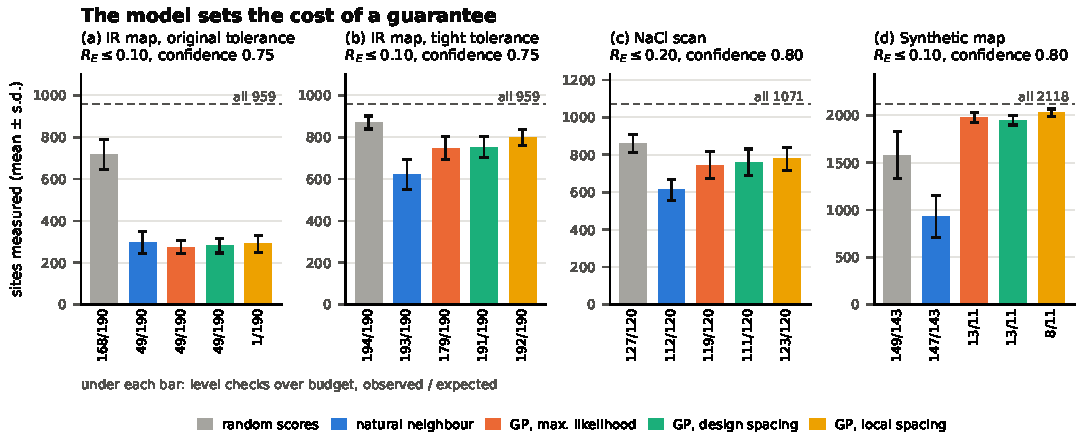
\includegraphics[width=\textwidth]{figures/fig_cost}
\caption{What a guarantee costs under different models: sites measured (mean \ensuremath{\pm} s.d. over 250 campaigns, quantile path) with random scores and with four interpolation protocols, against the number of design sites (dashed). Under each bar: level checks over budget on the shared rate, observed against expected under the picked failure probabilities. GP: Gaussian process with isotropic squared-exponential kernel; length scale by maximum likelihood, by design spacing, or by local spacing of measured sites.}\label{fig:6}
\end{figure}

\hypertarget{sec:5-5}{%
\subsection{The claim decides what is protected}\label{sec:5-5}}

Each claim protects what it states, so its choice deserves a record. Six acceptance metrics were compared on the three maps with the interpolation claim alone (SI 6). Every metric kept its guarantee, and the metric set the cost: at tolerances a practitioner might pick, the IR map needed between 233 and 810 measurements. At tolerances matched to equal difficulty the metric still decided where measurements went, with the peak claim on the synthetic map measuring where the peak drifts with composition and the profile claim along the phase boundaries (Fig. S6), and it decided where wrong skips fell. The rate counts wrong skips over all sites of a level; on the synthetic map 35 \% of the interesting sites on certified levels were skipped in error while every level met its budget (SI 6.2).

\hypertarget{sec:6}{%
\section{Discussion}\label{sec:6}}

\hypertarget{the-value-of-a-stated-rate}{%
\subsection{The value of a stated rate}\label{the-value-of-a-stated-rate}}

A stated rate is worth most where decisions rest on it: a budget chosen in advance holds at its confidence, and a model\textquotesingle s own statement missed by a factor of ten or more (Section~\ref{sec:5-2}). Accountability costs measurements; on the NaCl scan, certifying the Gaussian process took about 100 more in exchange for a rate fixed in advance and kept. The record adds a second value in failure. A level over budget is either chance at the stated rate or a sign that a condition of Section~\ref{sec:3-1} failed, through drift, beam damage or a draw that was not uniform, and the record tells which to examine. An uncertified agent leaves its errors unapportioned between model, data and chance.

\hypertarget{scope-of-the-guarantee}{%
\subsection{Scope of the guarantee}\label{scope-of-the-guarantee}}

A map built under a guarantee serves its reader to the extent that the reader knows what the bound covers. The bound concerns the share of wrong skips among all design sites of a level, with probability over the calibration draw. Section~\ref{sec:5-5} and SI 6 show the two consequences: wrong skips gather in space, and when signal is rare a budget met on every level can still cost a large share of the sites of interest. A bound on the share of interesting sites lost calls for a label-conditional statement, calibrated on the calibration sites that hold signal \cite{Vovk2005,Sadinle2019}. A uniform draw keeps those sites exchangeable with the interesting sites of the level, at the price of a calibration sample larger by the inverse of the share of interest; SI 9 gives the corresponding bound for the map. Calibration carries a fixed cost of 40 sites per certified level, up to a sixth of the IR map, a share that falls as maps grow, since the budget and the confidence alone set the sample size.

\hypertarget{what-is-certified-shapes-the-campaign}{%
\subsection{What is certified shapes the campaign}\label{what-is-certified-shapes-the-campaign}}

A guarantee is stated for one acceptance metric, and the metric deserves the same care as the budget. The bound holds for any metric fixed before the calibration draw, and the metric decides the rest: which sites fail prediction, where measurements are taken and where wrong skips gather (Section~\ref{sec:5-5}). The same holds for any autonomous experiment: the quantity a model predicts, and the error its acquisition anticipates, decide where measurements are taken \cite{Noack2019,Noack2020}. The guarantee delivers the claim as specified, and features outside that claim carry no protection. The metric is therefore best fixed from the scientific question before beam time, stated with the guarantee, and checked on a pilot scan for the cost it implies.

\hypertarget{extensions}{%
\subsection{Extensions}\label{extensions}}

The mechanism leaves wide freedom in the rules it certifies. Any score frozen before the draw keeps the bound, including one that ranks sites by the information they would add to a process model \cite{Atkinson2007}. Certification may bound any rate that counts sites, such as the share of interesting sites lost or a rate within groups of sites, and ratios such as the share of skips that are wrong are controlled through conformal p-values \cite{Jin2023}. Two conditions carry every such statement: the calibration sites are an exchangeable draw from the population the statement concerns, with a Mondrian category fixed before the draw taking the place of the level \cite{Vovk2005}, and the rule is non-anticipating (Section~\ref{sec:3-1}); each new form passes the Monte Carlo check of SI 4. A loss graded by the size of an error is not a count; for a bounded loss, confidence sequences for sampling without replacement \cite{WaudbySmith2020} give a bound of the same kind and would let calibration stop as soon as the bound is settled. Optimisation is the natural next case. Its proposals come from the model just fitted, and reweighting by the known selection mechanism \cite{Tibshirani2019,Fannjiang2022,Barber2023}, online control of a long-run rate \cite{Gibbs2021} and level sets, each a mapping problem with a threshold fixed before its draw \cite{CerouGuyader2007,Gotovos2013}, offer routes to a bound.

\hypertarget{accountable-experiments}{%
\subsection{Accountable experiments}\label{accountable-experiments}}

An accountable experiment certifies every action: each skip by its claim and bound, each measurement by the reason it was needed when the decision was made. The workflow leaves both in its record. Each site carries its level, scores and certified action; each level carries its calibration draw, picked failure probability and bound. The guarantee rests on the order of operations, so the record suffices: predictor and scores are frozen and recorded before each draw, the draw comes from a recorded seed, and every decision can be replayed, every bound recomputed (SI 5) and every measurement checked in hindsight (SI 8). The guarantee bounds, at the stated confidence, the share of each level skipped under a false claim. Claims, tolerances and budgets form the contract and remain the experimenter\textquotesingle s choice; the record shows that the contract was kept.

\begin{center}\rule{0.5\linewidth}{0.5pt}\end{center}

\hypertarget{sec:7}{%
\section{Conclusion}\label{sec:7}}

An experiment that leaves sites unmeasured can certify every action. A measurement is certified by the reason it was needed when the decision was made; a skip is certified by a claim about the site, calibrated on a uniform draw from a level of the plan fixed before the draw; the order fit, freeze, draw, calibrate, decide keeps each draw exchangeable with its level whatever came before. On three fully measured datasets the record matched the guarantees, with informed and random scores, natural-neighbour and Gaussian-process interpolation and three forms of guarantee. The model set the cost of a guarantee; trusted on its own uncertainty, the same model misstated its error rate. The certified claim decided what a guarantee bought: where measurements were taken, where wrong skips gathered and which sites were protected. The claim therefore belongs to the scientific question and enters the contract with it, before the experiment. Label-conditional bounds that protect the sites of interest, optimisation through level sets, scores that rank sites by the information they add to a process model, and deployment at autonomous instruments, beginning with a synthesis campaign, are natural next steps. Each skipped site leaves the campaign with a reason and a claim, each level with a bound, and the record allows every decision to be replayed.


\appendix
\hypertarget{app:A}{%
\section{Exchangeability by design and the single-certificate bound}\label{app:A}}

\hypertarget{conditions}{%
\subsection{Conditions}\label{conditions}}

A campaign processes the levels \(L = L_s + 1, L_s + 2, \dots\) of a hierarchical design in order. Write \(\mathcal{F}_{L-1}\) for everything known before the calibration draw of level \(L\): the design, the sites measured so far and their spectra, all earlier calibration draws, and any auxiliary randomness used by the scores. The truth \(y(x)\) at every design site is fixed; for a live experiment, \(y(x)\) is the outcome a measurement of \(x\) would return.

The order of operations of Section~\ref{sec:3-1} amounts to six conditions.

\begin{itemize}
\tightlist
\item
  \textbf{(A1) Fixed population.} The level population \(D_L\), of size \(N_L\), is determined by \(\mathcal{F}_{L-1}\). It may be declared before the experiment or drawn up from the sites measured so far; in this work the plan is declared in full before the experiment.
\item
  \textbf{(A2) Frozen scores and predictor.} The scores \(S_j\) and the predictor \(\hat y_L\) on \(D_L\) are determined by \(\mathcal{F}_{L-1}\).
\item
  \textbf{(A3) Labels.} Each bad label \(B_j(x)\), \(x \in D_L\), is a fixed function of the truth and of \(\hat y_L\), so the labels of the whole level are determined given \(\mathcal{F}_{L-1}\), whether or not a site is drawn.
\item
  \textbf{(A4) Fixed rule.} The family of covers searched (thresholds on one score, a path, a split of the budget), the budget \(\varepsilon\), the failure probability \(\delta\), the sample size \(m\) and the allowed number of failures \(k\) are determined by \(\mathcal{F}_{L-1}\).
\item
  \textbf{(A5) Uniform draw.} Given \(\mathcal{F}_{L-1}\), the calibration sample \(C_L\) is uniform over the \(m\)-subsets of \(D_L\).
\item
  \textbf{(A6) No interference.} Measuring a site of \(C_L\) leaves the truth at every other site unchanged.
\end{itemize}

Under (A1)--(A6), the level population with its scores and labels is a fixed finite population given \(\mathcal{F}_{L-1}\), and \(C_L\) is a simple random sample from it. Exchangeability of the calibration sites with the population is then a property of the draw \cite{Vovk2005}, and the bound below is a design-based statement \cite{Neyman1934,Cochran1977}: its only probability is that of the draw. The scores may depend on anything in \(\mathcal{F}_{L-1}\), including the truth itself through an oracle; such a score changes the cost and leaves the bound intact.

\hypertarget{the-bound}{%
\subsection{The bound}\label{the-bound}}

Fix a level and a certificate with score \(S\) and bad label \(B\), and drop the indices. The joint rate at threshold \(\tau\) is

\[
R(\tau) = N^{-1} \, \lvert \{x \in D : S(x) \le \tau,\ B(x) = 1\} \rvert
\]

which is nondecreasing and right-continuous in \(\tau\). Let \(H\) be hypergeometric with population \(N\), \(\lfloor \varepsilon N \rfloor + 1\) marked sites and \(m\) draws, and let \(k\) be the largest integer with \(P(H \le k) \le \delta\). Let \(b\) be the \((k+1)\)-th smallest score among the calibration sites with \(B = 1\). The rule covers every site with \(S < b\); every site when \(C\) holds at most \(k\) bad sites; no site when \(k < 0\).

\textbf{Proposition A.1.} Under (A1)--(A6),

\[
P\big(R(\hat\tau) > \varepsilon \mid \mathcal{F}_{L-1}\big) \le \delta_L = P(H \le k) \le \delta
\]

where \(\hat\tau\) is any threshold below \(b\) that covers the same sites.

\emph{Proof.} Condition on \(\mathcal{F}_{L-1}\); by (A1)--(A4) the population, scores, labels and \(k\) are fixed. Let \(\tau^\ast = \inf\{\tau : R(\tau) > \varepsilon\}\) and \(K = \{x : S(x) \le \tau^\ast,\ B(x) = 1\}\). By right-continuity \(|K| \ge \lfloor \varepsilon N \rfloor + 1\), and \(K\) does not depend on the draw. If \(R(\hat\tau) > \varepsilon\), then \(\hat\tau \ge \tau^\ast\), so every site of \(K\) has a score below \(b\). By construction at most \(k\) bad calibration sites have a score below \(b\), hence \(|C \cap K| \le k\). By (A5) and (A6), \(|C \cap K|\) is hypergeometric with \(|K|\) marked sites, and its lower tail decreases in \(|K|\):

\[
P\big(R(\hat\tau) > \varepsilon \mid \mathcal{F}_{L-1}\big) \le P\big(|C \cap K| \le k\big) \le P(H \le k)
\]

\(\square\)

The argument is the one-sided tolerance bound of Wilks (1941) in the form used for risk control \cite{Bates2021,Angelopoulos2025}, with the exact finite-population tail in place of its binomial approximation. The binomial \(k\), the largest with \(P(\mathrm{Bin}(m, \varepsilon) \le k) \le \delta\), is never larger and gives a valid, more conservative rule.

\textbf{The picked level.} \(\delta_L = P(H \le k)\) takes values on a grid indexed by \(k\) and set by \(m\), \(N_L\) and \(\varepsilon\). The rule picks the largest grid point at or below \(\delta\), and \(\delta_L\) is the failure probability the level asserts. Equality in Proposition A.1 holds when exactly \(\lfloor \varepsilon N \rfloor + 1\) bad sites lie at or below \(\tau^\ast\); Appendix~\ref{app:B}.5 describes the randomised rule that reaches \(\delta\) itself.

\textbf{Several levels.} Taking expectations over \(\mathcal{F}_{L-1}\) gives the unconditional bound on each level. For a statement about all certified levels at once, \(P(\exists L : R_L > \varepsilon) \le \sum_L \delta_L\).

\hypertarget{what-breaks-the-conditions}{%
\subsection{What breaks the conditions}\label{what-breaks-the-conditions}}

Each of the following lets the draw of a level shape the rule it is meant to test.

\begin{itemize}
\tightlist
\item
  \emph{Refitting on calibration labels} (breaks A2, A4). Scores updated with the calibration labels after the draw and then thresholded on the same labels. In the Monte Carlo of Section~\ref{sec:5-1} the bound was exceeded in every draw.
\item
  \emph{Choosing the calibration sites} (breaks A5). Calibrating where the scores are least sure, as an active learner would, makes the sample unrepresentative of the sites it speaks for.
\item
  \emph{Keeping the most favourable of several draws} (breaks A5). The retained sample is selected by its outcome.
\item
  \emph{Measurement-induced change} (breaks A6). Damage or drift caused by measuring the calibration sites alters the truth at their neighbours.
\end{itemize}

The sequential rule of Section~\ref{sec:5-1} breaks (A4) in a subtler way: its second threshold is searched over a family that depends on the labels the first threshold left uncovered.

\hypertarget{app:B}{%
\section{Guarantees on the shared wrong-skip event}\label{app:B}}

Fix a level with population \(D\) of \(N\) sites and a set \(J\) of certificates. Certificate \(j\) has a frozen score \(S_j\) and a bad label \(B_j\) (\(Z\) for interest, \(F\) for interpolation). A calibration sample \(C \subset D\) of size \(m\) is drawn uniformly without replacement after the scores are frozen; labels are known on \(C\) only. Write \(k(\varepsilon, \delta)\) for the largest integer with \(P(H \le k) \le \delta\), where \(H\) is hypergeometric with population \(N\), \(\lfloor \varepsilon N \rfloor + 1\) marked sites and \(m\) draws, as in Appendix~\ref{app:A}. The binomial tail \(P(\mathrm{Bin}(m, \varepsilon) \le k)\) gives a valid but smaller \(k\).

The shared wrong-skip event of a site under covers \(\{A_j\}\) is

\[
E(x) = \bigvee_{j \in J} \big(A_j(x) \wedge B_j(x)\big)
\]

and \(R_E = N^{-1} \sum_{x \in D} E(x)\).

\hypertarget{per-claim-budgets}{%
\subsection{Per-claim budgets}\label{per-claim-budgets}}

\textbf{Proposition B.1.} Let each \(\hat\tau_j\) be set by the rule of Appendix~\ref{app:A} with budget \(\varepsilon_j\) and failure probability \(\delta_j\), all on the same draw \(C\). Then, with probability at least \(1 - \sum_j \delta_j\),

\[
R_j(\hat\tau_j) \le \varepsilon_j \ \text{for every} \ j \in J
\]

and on the same event

\[
R_E \le \sum_{j \in J} \varepsilon_j
\]

\emph{Proof.} Appendix~\ref{app:A} bounds the probability of \(R_j(\hat\tau_j) > \varepsilon_j\) by \(\delta_j\) for each \(j\); the union bound over \(j\) gives the first statement. Since \(E(x) \le \sum_j A_j(x) B_j(x)\) for every site, \(R_E \le \sum_j R_j\). \(\square\)

On the same event, the rate of sites at which every covering claim fails is at most \(\min_j \varepsilon_j\). No threshold exists for certificate \(j\) when \(k(\varepsilon_j, \delta_j) < 0\), that is, when \(\varepsilon_j < 1 - \delta_j^{1/m}\); the certificate then covers nothing.

\hypertarget{one-budget-along-a-nested-path}{%
\subsection{One budget along a nested path}\label{one-budget-along-a-nested-path}}

A path is given by entry times \(\lambda_j(x) \in [0, \infty]\), one per certificate and site, computed from the frozen scores of the whole level and from settings fixed in advance, and from no calibration label. Certificate \(j\) covers \(x\) at path position \(\lambda\) when \(\lambda_j(x) \le \lambda\). Define the cover time and the failure time of a site,

\[
\lambda_{\mathrm{cov}}(x) = \min_{j \in J} \lambda_j(x)
\]

\[
\lambda_E(x) = \min \{\lambda_j(x) : j \in J,\ B_j(x) = 1\}
\]

with \(\lambda_E(x) = \infty\) when no label is bad. A site is a wrong skip at \(\lambda\) exactly when \(\lambda_E(x) \le \lambda\), so

\[
R_E(\lambda) = N^{-1} \, \lvert \{x \in D : \lambda_E(x) \le \lambda\} \rvert
\]

is nondecreasing and right-continuous in \(\lambda\). Let \(k = k(\varepsilon, \delta)\). Let \(b\) be the \((k+1)\)-th smallest finite value of \(\lambda_E\) on \(C\). The rule covers every site with \(\lambda_{\mathrm{cov}} < b\), every site when \(C\) holds at most \(k\) finite values of \(\lambda_E\), and no site when \(k < 0\). Write \(\hat\lambda\) for any position below \(b\) that covers the same sites.

\textbf{Proposition B.2.} With probability at least \(1 - \delta\) over the draw, \(R_E(\hat\lambda) \le \varepsilon\).

\emph{Proof.} Let \(\lambda^\ast = \inf\{\lambda : R_E(\lambda) > \varepsilon\}\). By right-continuity, the set \(K = \{x : \lambda_E(x) \le \lambda^\ast\}\) has \(|K| \ge \lfloor \varepsilon N \rfloor + 1\) sites. The set depends on the labels and the entry times, and on nothing drawn. If \(R_E(\hat\lambda) > \varepsilon\), then \(\hat\lambda \ge \lambda^\ast\), so every site of \(K\) has \(\lambda_E \le \hat\lambda\). Since \(\hat\lambda < b\), at most \(k\) calibration sites have \(\lambda_E \le \hat\lambda\), hence \(|C \cap K| \le k\). The count \(|C \cap K|\) is hypergeometric, and the remainder of the argument is that of Appendix~\ref{app:A}:

\[
P\big(R_E(\hat\lambda) > \varepsilon\big) \le P\big(|C \cap K| \le k\big) \le \delta
\]

\(\square\)

Testing the hypotheses \(R_E(\lambda) > \varepsilon\) in order of increasing \(\lambda\) and stopping at the first that cannot be rejected is fixed-sequence testing in Learn-then-Test \cite{Angelopoulos2025}; Proposition B.2 is the one-dimensional, monotone case. With a single certificate, \(\lambda_E\) and \(\lambda_{\mathrm{cov}}\) coincide on bad sites and the rule reduces to Appendix~\ref{app:A}.

\textbf{Quantile path.} With \(\hat F_j\) the empirical distribution function of \(S_j\) over the level and weights \(w_j \in (0, 1]\),

\[
\lambda_j(x) = \hat F_j(S_j(x)) / w_j
\]

\textbf{Priority path.} With \(i_j \in \{0, 1, \dots\}\) the position of certificate \(j\) in a fixed order,

\[
\lambda_j(x) = i_j + \hat F_j(S_j(x))
\]

so that certificate \(j\) sweeps its own quantiles over \(\lambda \in (i_j, i_j + 1]\) while earlier certificates stay at their final coverage. In both paths, a certificate restricted to sites below a cap on its score receives \(\lambda_j(x) = \infty\) above the cap. Both are functions of frozen scores and fixed settings, and Proposition B.2 applies.

\hypertarget{the-sequential-rule}{%
\subsection{The sequential rule}\label{the-sequential-rule}}

The rule of the original IR analysis first sets the interest threshold on \(C\), then sets the interpolation threshold on the calibration sites the interest certificate leaves uncovered, from the budget that remains. The second entry time then depends on calibration labels, \(K\) in the proof of Proposition B.2 is no longer fixed before the draw, and the hypergeometric step fails. Section~\ref{sec:5-1} reports the consequence on a population with uninformative scores: the bound is exceeded in 0.288 of draws against 0.25 allowed. The priority path keeps the same preference and the fixed-path condition.

\hypertarget{other-families}{%
\subsection{Other families}\label{other-families}}

Proposition B.2 needs a family of covers fixed before the labels and nested in one parameter. A family without that order, such as a two-dimensional grid of threshold pairs, is handled by Learn-then-Test with a family-wise correction across the grid \cite{Angelopoulos2025}, or by learning a path on one part of the draw and testing it on the other \cite{LauferGoldshtein2023}. Both give guarantees of the same kind at the cost of a smaller effective calibration sample.

\hypertarget{attaining-the-nominal-failure-probability}{%
\subsection{Attaining the nominal failure probability}\label{attaining-the-nominal-failure-probability}}

On a fixed level population, the exceedance probability of the rule above equals \(P(|C \cap K| \le k)\) when the wrong-skip rate crosses \(\varepsilon\) at exactly \(\lfloor \varepsilon N \rfloor + 1\) sites, and is smaller otherwise. With \(k\) from the hypergeometric tail, the bound is therefore attained up to the integer step in \(k\): at \(m = 40\) and \(\varepsilon = 0.10\), \(k = 2\) gives at most 0.21 on 399 sites against \(\delta = 0.25\). A randomised rule, which uses \(k + 1\) with the probability that makes the mixture of the two tails equal to \(\delta\), removes the step {[}Lehmann \& Romano 2005, ch. 3{]}. It makes the decision depend on an extra coin and is not used here.

\hypertarget{app:C}{%
\section{A bound on the conditional rate}\label{app:C}}

The rate bounded in Appendices A and B counts wrong skips among all sites of a level. A reader of the map may instead need the rate among the sites one claim covers. Learn then Test gives that bound for a family of thresholds fixed before the labels are seen \cite{Angelopoulos2025}.

Keep the notation of Appendix~\ref{app:B} for one certificate with frozen score \(S\) and bad label \(B\). The family of thresholds is a grid of quantiles of the frozen scores over the whole level,

\[
\tau_i = Q_S(q_i), \quad q_i = q_0 + 0.05\,(i - 1), \quad i = 1, \dots, I
\]

ending at \(q_I = 1\). Both the grid and \(q_0\) depend on the scores and on settings fixed in advance, and on no label. Threshold \(\tau_i\) covers the set \(D_i = \{x \in D : S(x) \le \tau_i\}\) of \(N_i\) sites, and its conditional rate is

\[
R_i = N_i^{-1} \, \lvert \{x \in D_i : B(x) = 1\} \rvert
\]

For each \(i\), the null hypothesis \(H_i : R_i > \alpha\) is tested on the calibration sites in \(D_i\). Their number \(n_i = |C \cap D_i|\) is random; given \(n_i\), they form a uniform sample without replacement from \(D_i\), since \(C\) is uniform on \(D\) and \(D_i\) is fixed before the draw. The number \(f_i\) of bad labels among them is then hypergeometric, and

\[
p_i = P(H_i^\ast \le f_i)
\]

with \(H_i^\ast\) hypergeometric on \(N_i\) sites, \(\lfloor \alpha N_i \rfloor + 1\) of them bad and \(n_i\) draws, is a valid p-value for \(H_i\) conditional on \(n_i\), hence also unconditionally. The binomial tail \(P(\mathrm{Bin}(n_i, \alpha) \le f_i)\) approximates it closely at the sizes of this study and is the one recorded.

The rates \(R_i\) need not increase with \(i\), so the hypotheses are tested in a fixed order: \(H_1, H_2, \dots\), each at level \(\delta\), stopping at the first that is not rejected. Fixed-sequence testing controls the family-wise error at \(\delta\) \cite{WestfallKrishen2001}, so with probability at least \(1 - \delta\) every rejected hypothesis is false. The rule covers \(D_{i^\ast}\), where \(i^\ast\) is the last rejection, and covers nothing when \(H_1\) is not rejected. With probability at least \(1 - \delta\),

\[
R_{i^\ast} \le \alpha
\]

\textbf{Minimum calibration size and starting quantile.} A hypothesis can be rejected only if its calibration sites can show a small enough tail even with no bad label, which requires \((1 - \alpha)^{n_i} \le \delta\), or

\[
n_i \ge n_{\min} = \lceil \log \delta / \log (1 - \alpha) \rceil
\]

The first threshold therefore covers at least the share \(n_{\min}/m\) of the level, and \(q_0\) is that share rounded up to a multiple of 0.05. With \(\alpha = \delta = 0.10\), \(n_{\min} = 22\), and at \(m = 40\) the grid starts at the 0.55 quantile: the rule certifies nothing or more than half of the level. A useful conditional bound thus calls for calibration samples several times larger than the rate bounds of Appendices A and B need, which is why the main text reports those.


% \ack{TODO}
% \funding{TODO}
% \roles{TODO}

\data{The NaCl microdiffraction scan is available from Dryad (doi:10.5061/dryad.p2ngf1w4t) \cite{ALSNaCl}. The following are deposited on Zenodo (doi:10.5281/zenodo.XXXXXXX, reserved): the infrared map of the bioreef sample as recorded and after scattering correction, with the hierarchical design used here; the forward model of the synthetic scattering map and its design; the run record of all 36 configurations, 250 campaigns each, with the decision and reason for every design site, the repeated calibration draws and the analyses of SI 6; and a snapshot of the software. The software provides the hierarchical design, natural-neighbour and Gaussian-process interpolation, the scores, the three forms of guarantee and the conditional rate, the map bound, the Monte Carlo acceptance check for new forms, the scattering correction for infrared maps, and the scripts that regenerate every figure and table from the record (SI 4).}

\suppdata{Supporting information: SI 1 interpolators; SI 2 dataset processing; SI 3 full tables; SI 4 adding a form of guarantee; SI 5 the run record; SI 6 the certified metric; SI 7 campaigns guided by Gaussian-process uncertainty; SI 8 the record of measured sites; SI 9 the map bound.}

\IfFileExists{iopart-num.bst}{\bibliographystyle{iopart-num}}{\bibliographystyle{unsrt}}
\bibliography{refs}

\end{document}
